\documentclass[a4paper,10pt]{article}
\usepackage{amsmath,amssymb}
\usepackage{minted}

\usepackage[numbers,sort&compress]{natbib}
\usepackage{minted}
\usepackage{url}
\usepackage{hyperref}
\usepackage{forest}

\title{User manual for Bernaise}
\author{Gaute Linga}

\begin{document}

\maketitle

%\begin{abstract}
\emph{Bernaise} (Binary Elect\textsc{r}ohydrody\textsc{na}m\textsc{i}c Solver) is a flexible high-level finite element solver of two-phase electrohydrodynamic flow in complex geometries.
\emph{Bernaise} is implemented in the Python interface to FEniCS, which effectively utilizes MPI and domain decomposition.
The software should therefore suitable for large-scale/high-performance computing.

In this document, we demonstrate briefly how to install \emph{Bernaise}, and how new solvers and problem set-ups can be implemented and added to the Bernaise framework by experienced Python users.
For the physical (and industrial) motivation, the underlying equations and a description of the solution schemes, we refer to the paper \cite{linga2018b}.

%\end{abstract}
\section{Prerequisites}
To work with \emph{Bernaise}, a basic familiarity with Python programming is needed.
Further, the user should be familiar with the finite element method (FEM) and how to solve partial differential equations (PDEs), in particular using FEM and FEniCS through the Python interface.
Otherwise, we refer readers to the tutorial by \citet{langtangen2017}.
Experience with the \emph{Oasis} flow solver \cite{mortensen2015}, which targets high-level/high-performance numerical solution of the Navier--Stokes equations, is also an advantage, since \emph{Bernaise} is inspired both in implementation and use of the latter.
You can find the \emph{Oasis} git repository on \url{github.com/mikaem/Oasis}.

On the software side, a working installation of Python 2.7 is needed, with the FEniCS/Dolfin package installed.
We refer to the FEniCS project's webpage \url{fenicsproject.org} for download and installation instructions.
Further, several other packages are required to benefit from the full functionality of Bernaise:
\begin{itemize}
\item \texttt{dolfin} and \texttt{mshr}: fundamental components (these are usually parts of the FEniCS install).
\item \texttt{numpy}: for calculations (necessary).
\item \texttt{scipy}: for analyzing/visualising data.
\item \texttt{simplejson}: for parsing the parameters.
\item \texttt{meshpy}: for generating periodic meshes.
\item \texttt{matplotlib}: for plotting/visualising data.
\item \texttt{argparse}: for some utility functionality.
\item \texttt{h5py} (parallel install): for accessing the output data.
\item \texttt{mpi4py}: for MPI.
\item \texttt{pytest}: for testing.
\item \texttt{scikit-image}: for utilities (mesh creation from images).
\end{itemize}

\section{Installation instructions}
You can install \emph{Bernaise} by cloning the Git repository (recommended) or by downloading a packaged version.
Packaged versions will be sought to be launched shortly after new stable versions of FEniCS.
At the time of writing, version 2017.2.0 is the latest stable FEniCS version, which is compatible with version 1.0 of \emph{Bernaise}.

\subsection{Installation via Git}
To install \emph{Bernaise} by cloning the GitHub repository.
\begin{minted}{bash}
>> git clone https://github.com/gautelinga/BERNAISE.git
>> cd BERNAISE
\end{minted}
To switch to, e.g., version 1.0 of \emph{Bernaise}, you can type:
\begin{minted}{bash}
>> git checkout v1.0
\end{minted}
which gives you the (as of writing) latest ``stable'' realease.

\subsection{Installation of the packaged version}
To install \emph{Bernaise} from a packaged file, you can navigate to \url{github.com/gautelinga/Bernaise/releases}.
In a Unix terminal, you can then install by performing the following commands:
\begin{minted}{bash}
>> wget https://github.com/gautelinga/Bernaise/archive/v1.0.tar.gz
>> tar -xvf v1.0.tar.gz
>> cd Bernaise-v1.0
\end{minted}

\subsection{Installing the dependencies}
The usually fastest way to install up-to-date dependencies is via \texttt{pip}:
\begin{minted}{bash}
>> pip install numpy scipy simplejson meshpy matplotlib \
>> argparse mpi4py pytest skimage
\end{minted}
Guides to install \texttt{h5py} in \emph{parallel} can be found several places on the web; one way is the following:
\begin{minted}{bash}
>> sudo apt-get install libhdf5-openmpi-10 libhdf5-openmpi-dev hdf5-tools
>> git clone https://github.com/h5py/h5py.git
>> cd h5py
>> git checkout 2.6.0 #(or a newer version)
>> export CC=mpicc.openmpi
>> python setup.py configure --mpi --hdf5=/usr/lib/x86_64-linux-gnu/hdf5/openmpi/
>> python setup.py build
>> sudo python setup.py install
\end{minted}
If you do not want to install systemwide, the last \texttt{sudo} can be skipped.

\section{Code structure}
\emph{Bernaise} is designed as a Python package, and its main executable script for running simulations is \texttt{sauce.py}.
For postprocessing, the main executable script is \texttt{postprocessing.py}.
The base level of the directory structure is shown in Fig.\ \ref{fig:dirtree}.

\begin{figure}[H]
  \begin{forest}
    for tree={
      font=\ttfamily,
      grow'=0,
      child anchor=west,
      parent anchor=south,
      anchor=west,
      calign=first,
      edge path={
        \noexpand\path [draw, \forestoption{edge}]
        (!u.south west) +(7.5pt,0) |- node[fill,inner sep=1.25pt] {} (.child anchor)\forestoption{edge label};
      },
      before typesetting nodes={
        if n=1
        {insert before={[,phantom]}}
        {}
      },
      fit=band,
      before computing xy={l=15pt},
    }
    [BERNAISE
      [README.md]
      [sauce.py]
      [postprocess.py]
      [common
        %[\_\_init\_\_.py]
        %[bcs.py]
        %[cmd.py]
        %[functions.py]
        %[io.py]
        [...]
      ]
      [problems
        %[\_\_init\_\_.py]
        %[charged\_droplet.py]
        %[taylorgreen.py]
        %[snoevsen.py]
        %[charged\_droplets\_3D.py]
        [...]
      ]
      [solvers
        %[\_\_init\_\_.py]
        %[basic.py]
        %[basicnewton.py]
        %[fracstep.py]
        [...]
      ]
      [utilities
        [...]
      ]
      [tests
        [...]
      ]
      [data
        [...]
      ]
      [meshes
        [...]
      ]
      [scripts
        [...]
      ]
      [analysis\_scripts
        [...]
      ]
      [...]
    ]
  \end{forest}
  \caption{\label{fig:dirtree}
    First level of the directory structure of Bernaise.}
\end{figure}

\subsection{\texttt{sauce.py}}
The task of the main module \texttt{sauce.py} is initializing the necessary variables to run a simulation, importing routines from the specified \texttt{problem} and \texttt{solver}, to iterate the solver in time, and to output and store data at appropriate times.
In particular, various \texttt{hooks} are called at various places in the code, where users can perform actions of choice within the code.

A simulation is typically run from a terminal, pointing to the \emph{Bernaise} directory, using the command
\begin{minted}[fontsize=\small]{bash}
>> python sauce.py problem=charged_droplet
\end{minted}
where \texttt{charged\_droplet} may be exchanged with another problem script of choice.
The main script \texttt{sauce.py} fetches a \texttt{problem}, from the folder \texttt{problems} (see below), and connects it with the \texttt{solver}, fetched from the folder \texttt{solvers} (see below).
It sets up the finite element problem with all the given parameters, initializes the finite element fields with the specified initial state, and solves it with the specified boundary condition at each time step, until the specified (physical) simulation time \texttt{T} is exceeded.

All default parameters in a problem by specifying an additional keyword from the command line; for example, the simulation time can be set to 1000 by running the command:

\begin{minted}[fontsize=\small]{bash}
>> python sauce.py problem=charged_droplet T=1000
\end{minted}

After every given interval of steps, specified by the parameter \texttt{save\_intv}, the simulation outputs XDMF/HDF5 data to a series of files.
The data structure is shown in Fig.\ \ref{fig:dirtree_data}.
The \texttt{Analysis} and \texttt{Plots} directories are reserved for post-processing.
\begin{figure}[H]
  \begin{forest}
    for tree={
      font=\ttfamily,
      grow'=0,
      child anchor=west,
      parent anchor=south,
      anchor=west,
      calign=first,
      edge path={
        \noexpand\path [draw, \forestoption{edge}]
        (!u.south west) +(7.5pt,0) |- node[fill,inner sep=1.25pt] {} (.child anchor)\forestoption{edge label};
      },
      before typesetting nodes={
        if n=1
        {insert before={[,phantom]}}
        {}
      },
      fit=band,
      before computing xy={l=15pt},
    }
    [results\_charged\_droplet
      [1
        [Checkpoint
          [fields.h5]
          [parameters.dat]
        ]
        [Timeseries
          [u\_from\_tstep\_0.xdmf]
          [u\_from\_tstep\_0.h5]
          [p\_from\_tstep\_0.xdmf]
          [p\_from\_tstep\_0.h5]
          [...]
        ]
        [Statistics]
        [Settings
          [parameters\_from\_tstep\_0.dat]
        ]
        [Analysis]
        [Plots]
      ]
    ]
  \end{forest}
  \caption{\label{fig:dirtree_data}
    Directory structure of the results.}
\end{figure}

After every given interval of steps, specified by the parameter \texttt{checkpoint\_interval}, a checkpoint is stored, including all fields, and all problem parameters at the time of writing to file.
The checkpoint can be loaded, and the simulation can be continued, by running the command:
\begin{minted}[fontsize=\small]{bash}
>> python sauce.py problem=charged_droplet \
   restart_folder=results_charged_droplet/1/Checkpoint/
\end{minted}
where the \texttt{restart\_folder} points to an appropriate checkpoint folder.
Here, the problem parameters stored within the checkpoint have precedence over the default parameters given in the \texttt{problem} script.
Further, any parameters specified by command line keywords have precedence over the checkpoint parameters.

If you want stop a simulation in a safe way while it is running, and ask it to save its current state, you can simply \texttt{kill} it smoothly:
\begin{minted}{bash}
>> touch results_charged_droplet/1/kill
\end{minted}

\subsection{\texttt{problems}}
The \texttt{problems} submodule (in the folder \texttt{problems}) contains the various problems that can be run in \emph{Bernaise}.
An incomplete list of problems that are currently implemented is shown in Fig.\ \ref{fig:dirtree_problems}.
\begin{figure}[H]
  \begin{forest}
    for tree={
      font=\ttfamily,
      grow'=0,
      child anchor=west,
      parent anchor=south,
      anchor=west,
      calign=first,
      edge path={
        \noexpand\path [draw, \forestoption{edge}]
        (!u.south west) +(7.5pt,0) |- node[fill,inner sep=1.25pt] {} (.child anchor)\forestoption{edge label};
      },
      before typesetting nodes={
        if n=1
        {insert before={[,phantom]}}
        {}
      },
      fit=band,
      before computing xy={l=15pt},
    }
    [problems
      [\_\_init\_\_.py]
      [charged\_droplet.py]
      [charged\_droplets.py]
      [charhed\_droplets\_3D.py]
      [taylorgreen.py]
      [snoevsen.py]
      [charged\_droplets\_3D.py]
      [barbell\_capilar.py]
      [dielectric.py]
      [dolphin.py]
      [electrowetting.py]
      [hourglass.py]
      [intrusion\_bulk.py]
      [porous.py]
      [simple.py]
      [simple\_3D.py]
      [single\_cell.py]
      [single\_reaction.py]
      [single\_taylorgreen.py]
      [...]
      ]
  \end{forest}
  \caption{\label{fig:dirtree_problems}
    The directory structure of the \texttt{problems} submodule.}
\end{figure}

Code that is shared between various solvers, in particular default values of the \texttt{hooks}, are placed in the top level \texttt{\_\_init\_\_.py} script.
For example, a list of ``base elements'' is defined:
\begin{minted}{python}
# Default base elements
# Format: name : (family, degree, is_vector)
base_elements = dict(u=["Lagrange", 2, True],
                     p=["Lagrange", 1, False],
                     phi=["Lagrange", 1, False],
                     g=["Lagrange", 1, False],
                     c=["Lagrange", 1, False],
                     V=["Lagrange", 1, False],
                     p0=["Real", 0, False],
                     c0=["Real", 0, False],
                     V0=["Real", 0, False])
\end{minted}
This \texttt{dict} defines which finite elements are automatically created by the \texttt{sauce.py} script (and can be overruled in the particular \texttt{problem}). 

A list of default \texttt{parameters} is also defined:
\begin{minted}{python}
# Set default parameters
parameters = dict(
    folder="results",  # default folder to store results in
    info_intv=10,
    use_iterative_solvers=False,
    use_pressure_stabilization=False,
    dump_subdomains=False,
    V_lagrange=False,
    p_lagrange=False,
    base_elements=base_elements,
    c_cutoff=0.,
    q_rhs=dict(),
    EC_scheme="NL2",
    grav_dir=[1., 0],
    pf_mobility_coeff=1.,
    grav_const=0.,
    surface_tension=0.,
    interface_thickness=0.,
    reactions=[],
    density_per_concentration=None,
    viscosity_per_concentration=None,
    testing=False,
    tstep=0
)
\end{minted}
We will not go into detail on the meaning of all these entries; they should be explained in the source code or in \cite{linga2018b}.
These can also be overruled in a \texttt{problem}; in particular, the function \texttt{problem} in any problem script is required to return a \texttt{dict}.
We shall look at a concrete example in Sec.\ \ref{sec:test_problem}.

Further, the following functions can be overruled:
\begin{itemize}
\item \texttt{constrained\_domain}: Returns e.g. periodic domain.
\item \texttt{initialize}: Initialize solution, i.e., the initial conditions.
\item \texttt{create\_bcs}: Returns a \texttt{dict} of Dirichlet boundary conditions.
\item \texttt{start\_hook}: Called just before entering the time loop.
\item \texttt{tstep\_hook}: Called in the beginning of timestep loop.
\item \texttt{end\_hook}: Called just before program ends.
\item \texttt{import\_problem\_hook}: Called after importing problem.
\item \texttt{rhs\_source}: for adding source terms, e.g., for validation purposes.
\item \texttt{pf\_mobility}: default phase field mobility function (see \cite{linga2018b}).
\end{itemize}
Note that all of these functions (with the exception of \texttt{pf\_mobility}) can import \emph{any parameter returned by the} \texttt{problem} \emph{function}, which will be exemplified in Sec.\ \ref{sec:test_problem}.

\subsection{\texttt{solvers}}
Similarly to the \texttt{problems} submodule, there are several solvers implemented in the \texttt{solvers} module.
In particular, a solver can be defined in the \texttt{dict} returned by the \texttt{problem} function in a problem, or it can be set from the command line by running:
\begin{minted}{bash}
>> python sauce.py problem=charged_dropet solver=basicnewton
\end{minted}
if, by chance, we wanted to use the \texttt{basicnewton} scheme instead of \texttt{basic}.
A list of implemented solver is shown Fig.\ \ref{fig:dirtree_solvers}.
\begin{figure}[H]
  \begin{forest}
    for tree={
      font=\ttfamily,
      grow'=0,
      child anchor=west,
      parent anchor=south,
      anchor=west,
      calign=first,
      edge path={
        \noexpand\path [draw, \forestoption{edge}]
        (!u.south west) +(7.5pt,0) |- node[fill,inner sep=1.25pt] {} (.child anchor)\forestoption{edge label};
      },
      before typesetting nodes={
        if n=1
        {insert before={[,phantom]}}
        {}
      },
      fit=band,
      before computing xy={l=15pt},
    }
    [solvers
      [\_\_init\_\_.py]
      [basic.py]
      [basicnewton.py]
      [fracstep.py]
      [stable\_single.py]
      [stable\_single\_fracstep.py]
      [...]
      ]
  \end{forest}
  \caption{\label{fig:dirtree_solvers}
    The directory structure of the \texttt{solvers} submodule.}
\end{figure}
\texttt{basic} is a semi-implicit operator splitting scheme, that solves sequentially the three linearized subproblems of fluid flow, phase field propagation and electrochemistry at each time step.
\texttt{basicnewton} is a fully implicit monolithic scheme, which solves the whole coupled problem using a Newton method.
\texttt{fracstep} is a variant of \texttt{basic} that is fully iterative and more scalable, in that it further splits the fluid flow step with a projection method.
The solvers that start with the name \texttt{stable\_single} only support single-phase flow, and have been documented in Ref.\ \cite{linga2018decoupled}.

Code that is shared across the different solvers is defined in the top level file \texttt{\_\_init\_\_.py}.
In common with its counterpart in the \texttt{problems} submodule, \texttt{\_\_init\_\_.py} defines a set of placeholder functions that should be overloaded in the specific \texttt{solver} instance.
\begin{itemize}
\item \texttt{get\_subproblems}: Returns \texttt{dict} of subproblems as defined by the solver.
\item \texttt{setup}: Sets up all equations that should be solved.
  Returns \texttt{dict} of solvers.
\item \texttt{solve}: Solves equations at each timestep.
\item \texttt{update}: Update work arrays at the end of timestep.
\end{itemize} 
We will examplify these for the \texttt{basic} solver in Sec.\ \ref{sec:basic_solver}.

\subsection{\texttt{utilities}}
\emph{Bernaise} comes with a set of utility scripts that are located in the \texttt{utilities} folder.
This subdirectory is shown Fig.\ \ref{fig:dirtree_utilities}.
\begin{figure}[H]
  \begin{forest}
    for tree={
      font=\ttfamily,
      grow'=0,
      child anchor=west,
      parent anchor=south,
      anchor=west,
      calign=first,
      edge path={
        \noexpand\path [draw, \forestoption{edge}]
        (!u.south west) +(7.5pt,0) |- node[fill,inner sep=1.25pt] {} (.child anchor)\forestoption{edge label};
      },
      before typesetting nodes={
        if n=1
        {insert before={[,phantom]}}
        {}
      },
      fit=band,
      before computing xy={l=15pt},
    }
    [utilities
      [extract\_polygons.py]
      [generate\_mesh.py]
      [get\_info.py]
      [TimeSeries.py]
      [...]
      ]
  \end{forest}
  \caption{\label{fig:dirtree_utilities}
    The directory structure of the \texttt{utilities} submodule.}
\end{figure}

Here, \texttt{generate\_mesh.py} is somewhat similar to \texttt{sauce.py} in that it pulls in a required mesh generation script from the folder \texttt{utilities/mesh\_scripts}.
For example, an hourglass mesh can be generated by navigating into the \texttt{utilities} folder and running the command:
\begin{minted}{bash}
>> python generate_mesh.py mesh=hourglass
\end{minted}
An hourglass mesh will then be created in the \texttt{meshes} folder (see Fig.\ \ref{fig:dirtree}).
Different parameters than the default ones can be set by adding supplying keywords in the command-line interface.
An incomplete list of meshes that can be generated, and thus are stored in the latter folder, is the following:
\begin{itemize}
\item \texttt{barbell\_capilar}
\item \texttt{extended\_polygon}
\item \texttt{hourglass}
\item \texttt{periodic\_porous}
\item \texttt{snoevsen}
\item \texttt{straight\_capilar}
\end{itemize}
To get an overview of all implemented mesh scripts, and their possible parameters, you can run:
\begin{minted}{bash}
>> python generate_mesh.py -h
\end{minted}
\texttt{extract\_polygons.py} is a small script for extracting shapes (as polygons) from images, to produce meshes from them.
It should be used as
\begin{minted}{bash}
>> python extract_polygons.py image=(path to image)
\end{minted}
\texttt{get\_info.py} is a small script for quickly getting parameters from a simulation that has been run, without inspecting manually the JSON output file (\texttt{parameters.dat}).
It can be run as:
\begin{minted}{bash}
>> python get_info.py folder=(path to output directory)
\end{minted}
\texttt{TimeSeries.py} is fundamental for the post-processing procedures (i.e., reading XDMF/HDF5 files), which will be covered in Sec.\ \ref{sec:postproc}.

\subsection{Post-processing}
\label{sec:postproc}
The post-processing executable \texttt{postprocessing.py} connects to a range of practical tools for efficient analysis of simulation output.
These scripts are (similarly to \texttt{problems} and \texttt{solvers}) found in the \texttt{analysis\_scripts} folder.
At the present, some of these only work in two dimensions (2D), but most of the tools should be functional also with three-dimensional simulations.
The directory structure is shown in Fig.\ \ref{fig:dirtree_analysis}.
\begin{figure}[H]
  \begin{forest}
    for tree={
      font=\ttfamily,
      grow'=0,
      child anchor=west,
      parent anchor=south,
      anchor=west,
      calign=first,
      edge path={
        \noexpand\path [draw, \forestoption{edge}]
        (!u.south west) +(7.5pt,0) |- node[fill,inner sep=1.25pt] {} (.child anchor)\forestoption{edge label};
      },
      before typesetting nodes={
        if n=1
        {insert before={[,phantom]}}
        {}
      },
      fit=band,
      before computing xy={l=15pt},
    }
    [analysis\_scripts
      [\_\_init\_\_.py]
      [analytic\_reference.py]
      [boundary\_value\_in\_time.py]
      [energy\_in\_time.py]
      [flux\_in\_time.py]
      [geometry\_in\_time.py]
      [line\_probe.py]
      [make\_gif.py]
      [mesh.py]
      [plot.py]
      [plot\_dolfin.py]
      [reference.py]
      [value\_in\_time.py]
      [...]
    ]
  \end{forest}
  \caption{\label{fig:dirtree_analysis}
    Directory structure of the \texttt{analysis\_scripts}.}
\end{figure}
To get an overview over all implemented analysis scripts, you can run:
\begin{minted}{bash}
>> python postprocess.py method=analytic_reference folder=results_taylorgreen/1/
\end{minted}
if, say, you wanted to compare your Taylor--Green vortex results against an analytic reference.
(Note that there needs to be a \texttt{reference} function, which gives FEniCS \texttt{Expression}s for the analytical refernce solutions, in the \texttt{problem} in order for this function to work.)

The various analysis scripts can be detailed by running the command
\begin{minted}{bash}
>> python postprocess.py method=analytic_reference?
\end{minted}
or similarly for other scripts.
This basically calls the \texttt{description} function defined within an \texttt{analysis\_script} instead of the \texttt{method} function.
Again, we request the interested or experimentally-minded users to have a look directly into the source code for examples and a more in-depth insight.

\subsection{common/bcs.py}
\label{subsec:bernaise_bcs}
Boundary conditions are among the few components of \emph{Bernaise} which are implemented as classes.
The boundaries definitions should be set by the user within the \texttt{problem} in the standard Python way.
By importing various boundary condition classes from \texttt{common/bcs.py}, the boundary conditions can be inferred at user-specified boundaries.

Within the \texttt{bcs} module, the base class \texttt{GenericBC} is defined.
The boolean member functions \texttt{is\_dbc} and \texttt{is\_nbc} specifies, respectively, whether the concrete boundary conditions impose a Dirichlet and Neumann condition, and both return false by default.
The base class is inherited by various concrete boundary conditon classes, and by overloading these two member functions, the member functions \texttt{dbc} or \texttt{nbc} are respectively called at appropriate times in the code.

There is a hierarchy of boundary conditions which inherit from each other.
An incomplete list of implemented boundary conditions in \emph{Bernaise} are:
\begin{itemize}
\item \texttt{GenericBC}: Base class for all boundary conditions.
  \begin{itemize}
  \item \texttt{Fixed}: Dirichlet condition, applicable for all fields.
    \begin{itemize}
    \item \texttt{NoSlip}: The no-slip condition---a pure Dirichlet condition with the value $\mathbf 0$, applicable for velocity.
    \item \texttt{Pressure}: Constant pressure boundary condition---adds a Neumann condition to the velocity, i.e.~a boundary term in the variational form.
    \end{itemize}
  \item \texttt{Charged}: A charged boundary---a Neumann conditon intended for use with the electric potential $V$.
  \end{itemize}
\end{itemize}

\section{The \texttt{basic} solver}
\label{sec:basic_solver}
Now we briefly explain the implementation of the \texttt{basic} solver.
This is intended only as a brief outline; users who would like to implement or experiment with their own schemes, should also look in the source code and the in-line documentation.

\subsection{\texttt{get\_subproblems}}
The overloaded \texttt{get\_subproblems} function in \texttt{basic} consists of:
\begin{minted}{python}
def get_subproblems(base_elements, solutes, p_lagrange,
                    enable_NS, enable_PF, enable_EC,
                    **namespace):
    subproblems = dict()
    if enable_NS:
        subproblems["NS"] = [dict(name="u", element="u"),
                             dict(name="p", element="p")]
        if p_lagrange:
           subproblems["NS"].append(dict(name="p0",
                                         element="p0"))
    if enable_PF:
        subproblems["PF"] = [dict(name="phi", element="phi"),
                             dict(name="g", element="g")]
    if enable_EC:
        subproblems["EC"] = ([dict(name=solute[0], element="c")
                              for solute in solutes]
                             + [dict(name="V", element="V")])
    return subproblems
\end{minted}
First, note that any parameter that has been defined in the namespace, can inter into the list of arguments.
Here, \texttt{base\_elements} were defined in the \texttt{problem} that has called the \texttt{basic} solver, and the entries of the \texttt{subproblems} \texttt{dict} are the subproblems that the solver splits the full problem into, here \texttt{NS} (Navier--Stokes), \texttt{PF} (phase field) and \texttt{EC} (electrochemistry).
Within each entry, a list of \texttt{dict}s that make up mixed finite elements is specified.
The \texttt{name} key gives the name of the field and \texttt{element} points to the element whose key is the value.
The \texttt{solutes} parameter is an array of arrays which give (1) name, (2) valency, (3) diffusivity in phase 1, (4) diffusivity in phase 2, (5) solubility energy in phase 1, and (6) solubility energy in phase 2.
See Sec.\ \ref{sec:test_problem} for an example.
The boolean parameter \texttt{p\_lagrange} states whether a Lagrange multiplier should be used to fix the pressure gauge (this enters as an additional degree of freedom in the subproblem).
The parameters \texttt{enable\_NS}, \texttt{enable\_PF}, and \texttt{enable\_EC} are boolean values that determine whether the various subproblems should be enabled.

\subsection{\texttt{setup}}
The main structure of the \texttt{setup} function is given as:
\begin{minted}{python}
def setup(test_functions, trial_functions,
          w_, w_1,
          ds, dx, normal,
          dirichlet_bcs, neumann_bcs, boundary_to_mark,
          permittivity, density, viscosity, solutes,
          enable_PF, enable_EC, enable_NS,
          surface_tension, dt, interface_thickness,
          grav_const, grav_dir, pf_mobility, pf_mobility_coeff,
          p_lagrange, q_rhs,
          **namespace):

    ... #(unpack values from work arrays to mathematical symbols)
          
    solvers = dict()
    if enable_PF:
        solvers["PF"] = setup_PF(
           w_["PF"], phi, g, psi, h, dx, ds,
           dirichlet_bcs["PF"],
           neumann_bcs, boundary_to_mark, phi_1,
           u_1, M_1, c_1, V_1,
           per_tau, sigma_bar, eps, dbeta, dveps,
           enable_NS, enable_EC, use_iterative_solvers, q_rhs)

    if enable_EC:
        solvers["EC"] = setup_EC(
           w_["EC"], c, V, b, U, rho_e, dx, ds,
           dirichlet_bcs["EC"],
           neumann_bcs, boundary_to_mark, c_1, u_1, K_,
           veps_, phi_flt_, solutes, per_tau, z, dbeta,
           enable_NS, enable_PF, use_iterative_solvers, q_rhs)

    if enable_NS:
        solvers["NS"] = setup_NS(
           w_["NS"], u, p, v, q, p0, q0, dx, ds, normal,
           dirichlet_bcs["NS"], neumann_bcs, boundary_to_mark,
           u_1, phi_flt_, rho_, rho_1, g_, M_, mu_, rho_e_,
           c_, V_, c_1, V_1, dbeta, solutes,
           per_tau, drho, sigma_bar, eps, dveps, grav,
           enable_PF, enable_EC, use_iterative_solvers,
           use_pressure_stabilization, p_lagrange, q_rhs)
    return dict(solvers=solvers)
\end{minted}
Here, it is important to note the significance of \texttt{setup}: it is to unwrap the values from the vectors in \texttt{w\_} (present value of all fields), \texttt{w\_1} (previous time step value), \texttt{test\_functions} (test functions), and \texttt{trial\_functions} (trial functions).
The fields within \texttt{w\_}, etc., are accessed by subproblem name.
For example, velocity and pressure trial and test functions are retrieved by:
\begin{minted}{python}
if enable_NS:
   u, p = trial_functions["NS"][:2]
   v, q = test_functions["NS"][:2]
\end{minted}
For convenience, setting up the variational forms are ``outsourced'' to the separate subroutines \texttt{setup\_NS}, \texttt{setup\_PF}, and \texttt{setup\_EC}, which are all placed in the same solver script \texttt{basic.py}. 
(In principle, they could have been taken from other files, as well.)
In the end, \texttt{setup} returns a \texttt{dict} of solvers.

We show as an example the very \texttt{basic} implementation of the \texttt{setup\_PF} subroutine below:
\begin{minted}{python}
def setup_PF(w_PF, phi, g, psi, h, dx, ds,
             dirichlet_bcs, neumann_bcs, boundary_to_mark,
             phi_1, u_1, M_1, c_1, V_1,
             per_tau, sigma_bar, eps, dbeta, dveps,
             enable_NS, enable_EC, use_iterative_solvers, q_rhs):
    """ Set up phase field subproblem. """

    F_phi = (per_tau*(phi-unit_interval_filter(phi_1))*psi*dx +
             M_1*df.dot(df.grad(g), df.grad(psi))*dx)
    if enable_NS:
        F_phi += -phi*df.dot(u_1, df.grad(psi))*dx
    F_g = (g*h*dx
           - sigma_bar*eps*df.dot(df.nabla_grad(phi),
                                  df.nabla_grad(h))*dx
           - sigma_bar/eps*(
               diff_pf_potential_linearised(phi,
                                            unit_interval_filter(
                                                phi_1))*h*dx))
    if enable_EC:
        F_g += (-sum([dbeta_i*ci_1*h*dx
                      for dbeta_i, ci_1 in zip(dbeta, c_1)])
                      + 0.5*dveps*df.dot(df.nabla_grad(V_1),
                                         df.nabla_grad(V_1))*h*dx)

    for boundary_name, costheta in neumann_bcs["phi"].iteritems():
        fw_prime = diff_pf_contact_linearised(
            phi, unit_interval_filter(phi_1))
        F_g += sigma_bar*costheta*fw_prime*h*ds(
            boundary_to_mark[boundary_name])

    if "phi" in q_rhs:        
        F_phi += -q_rhs["phi"]*psi*dx
    
    F = F_phi + F_g
    a, L = df.lhs(F), df.rhs(F)

    problem = df.LinearVariationalProblem(a, L, w_PF)
    solver = df.LinearVariationalSolver(problem)

    if use_iterative_solvers:
        solver.parameters["linear_solver"] = "gmres"
        solver.parameters["preconditioner"] = "jacobi"
    
    return solver
\end{minted}
This implementation is meant to be simple and humanly readable.
For the scheme and meaning of the symbols, we refer to \cite{linga2018b}.

\subsection{\texttt{solve}}
Within each time step, a call is given to \texttt{solve}, which accesses the \texttt{solvers} \texttt{dict} created in the \texttt{setup} step.
The overloaded version in the \texttt{basic} solver is given by:
\begin{minted}{python}
def solve(w_, solvers, enable_PF, enable_EC, enable_NS, **namespace):
    """ Solve equations. """
    timer_outer = df.Timer("Solve system")
    for subproblem, enable in zip(["PF", "EC", "NS"],
                                  [enable_PF, enable_EC, enable_NS]):
        if enable:
            timer_inner = df.Timer("Solve subproblem " + subproblem)
            df.mpi_comm_world().barrier()
            solvers[subproblem].solve()
            timer_inner.stop()

    timer_outer.stop()
\end{minted}
Note that some timers are accessed within this loop, in order to inspect the runtimes.
This subroutine is not expected to return anything.

\subsection{\texttt{update}}
At the end of each time step, it is in place to update the work variables, i.e.\ increase the time step counter.
In the \texttt{basic} solver, this is done as follows.
\begin{minted}{python}
def update(t, dt, w_, w_1, bcs, bcs_pointwise,
           enable_PF, enable_EC, enable_NS, q_rhs, **namespace):
    """ Update work variables at end of timestep. """
    # Update the time-dependent source terms
    for qi in q_rhs.values():
        qi.t = t+dt
    # Update the time-dependent boundary conditions
    for boundary_name, bcs_fields in bcs.iteritems():
        for field, bc in bcs_fields.iteritems():
            if isinstance(bc.value, df.Expression):
                bc.value.t = t+dt

    # Update fields
    for subproblem, enable in zip(
        ["PF", "EC", "NS"],
        [enable_PF, enable_EC, enable_NS]):
        if enable:
            w_1[subproblem].assign(w_[subproblem])
\end{minted}
Note that here, the time-dependent source terms in \texttt{q\_rhs}, and boundary conditions, are updated to represent the correct time.

\section{How do I implement a new \texttt{problem}?}
The essentials of implementing a new problem consists of the following points, which all need to be addressed properly in a file placed within the \texttt{problems} subdirectory.
\begin{itemize}
\item Specify a mesh.
  This requires you to set the \texttt{mesh} variable (function or Dolfin mesh).
\item Specify boundary conditions.
\item Initial conditions.
\item Physical parameters.
\end{itemize}
You might also want to use one or more of the \texttt{hooks} to do post-processing.
Alternatively, the built-in post-processing tool works directly on the XDMF/HDF5 output.

We will in the following section demonstrate for an example problem how these parts are implemented.

\subsection{Charged droplet in an electric field}
\label{sec:test_problem}
We consider now the test problem of a charged droplet driven by an electric field, which was described in detail in \cite{linga2018b}.

On the top of the file, we import the necessary packages and routines from other files in \emph{Bernaise}.
\begin{minted}{python}
import dolfin as df
import os
from . import *
from common.io import mpi_is_root
from common.bcs import Fixed
__author__ = "Gaute Linga"

class Wall(df.SubDomain):
    def __init__(self, Lx):
        self.Lx = Lx
        df.SubDomain.__init__(self)

    def inside(self, x, on_boundary):
        return bool(x[0] >= df.DOLFIN_EPS and
                    x[0] <= self.Lx-df.DOLFIN_EPS and on_boundary)

class Left(df.SubDomain):
    def inside(self, x, on_boundary):
        return bool(x[0] < df.DOLFIN_EPS and on_boundary)

class Right(df.SubDomain):
    def __init__(self, Lx):
        self.Lx = Lx
        df.SubDomain.__init__(self)

    def inside(self, x, on_boundary):
        return bool(x[0] > self.Lx-df.DOLFIN_EPS and on_boundary)
\end{minted}
Note how the subdomains \texttt{Left} and \texttt{Wall} are allowed to import the dimensions of the domain, \texttt{Lx} and \texttt{Ly}.

Next, we should define the main function \texttt{problem}, which overrides the default parameters.
Here, the \texttt{solutes} array (which defines the solutes), contains only one species, but it can in principle contain arbitrarily many.
\begin{minted}[fontsize=\small]{python}
def problem():
    info_cyan("Charged droplet in an electric field.")

    # Define solutes
    # Format: name, valency, diffusivity in phase 1, diff. in ph. 2,
    #         solubility energy in phase 1, sol. en. in phase 2
    solutes = [["c_p",  1, 1e-5, 1e-3, 4., 1.]]

    # Default parameters to be loaded unless starting from checkpoint.
    parameters = dict(
        solver="basic",                    # Solver to be used.
        folder="results_charged_droplet",  # Folder to store results
        dt=0.08,                           # Timestep
        t_0=0.,                            # Starting time
        T=8.,                              # Total simulation time
        grid_spacing=1./32,                # Mesh size
        interface_thickness=0.03,          # Extent of diff. interface
        solutes=solutes,                   # Array of solutes
        Lx=2.,                             # Length of domain along x
        Ly=1.,                             # Length of domain along y
        rad_init=0.25,                     # Initial droplet radius
        V_left=10.,                        # Potential at left side
        V_right=0.,                        # Potential at right side
        surface_tension=5.,                # Surface tension
        concentration_init=10.,            # Initial (total) conc.
        pf_mobility_coeff=0.00002,         # Phase field mob. coeff.
        density=[200., 100.],              # Density in ph. 1, ph. 2
        viscosity=[10., 1.],               # Viscosity in ph. 1, ph. 2
        permittivity=[1., 1.]              # Permittivity in ph 1, ph 2
    )
    return parameters
\end{minted}
The description of the parameters that enter here are shown as inline comments.

The \texttt{mesh} function should also be defined.
In this case, it is rather easy:
\begin{minted}{python}
def mesh(Lx=1, Ly=5, grid_spacing=1./16, **namespace):
    m = df.RectangleMesh(df.Point(0., 0.), df.Point(Lx, Ly),
                         int(Lx/(2*grid_spacing)),
                         int(Ly/(2*grid_spacing)))
    m = df.refine(m)
    return m
\end{minted}
(The \texttt{df.refine} command was used once to make the mesh symmetric.)

Next, all fields should be initialized, otherwise they will be set to zero by default.
This is done through the \texttt{initialize} command.
\begin{minted}{python}
def initialize(Lx, Ly, rad_init, interface_thickness, solutes,
               concentration_init, restart_folder,
               field_to_subspace,
               enable_NS, enable_PF, enable_EC, **namespace):
    """ Create the initial state. """
    w_init_field = dict()
    if not restart_folder:
        x0, y0, rad0, c0 = Lx/4, Ly/2, rad_init, \
            concentration_init
        # Initialize phase field
        if enable_PF:
            w_init_field["phi"] = initial_pf(
                x0, y0, rad0, interface_thickness,
                field_to_subspace["phi"].collapse())

        # Initialize electrochemistry
        if enable_EC:
            w_init_field[solutes[0][0]] = initial_c(
                x0, y0, rad0/3., c0, interface_thickness,
                field_to_subspace[solutes[0][0]].collapse())

    return w_init_field
\end{minted}
Note here how \texttt{field\_to\_subspace} is used extensively to relate the field to the subspace which the function should be projected to.  
Here, the two ``outsourced'' initialization functions, defined in the problem, are given by:
\begin{minted}{python}
def initial_pf(x0, y0, rad0, eps, function_space):
    """ Function describing the initial phase field. """
    expr_str = ("1.-(1.-tanh(sqrt(2)*(sqrt(pow(x[0]-{x}, 2)"
                "+pow(x[1]-{y}, 2))-{rad})/{eps}))").format(
                    x=x0, y=y0, rad=rad0, eps=eps)
    phi_init_expr = df.Expression(expr_str, degree=2)
    phi_init = df.interpolate(phi_init_expr, function_space)
    return phi_init
    
def initial_c(x, y, rad, c_init, eps, function_space):
    """ Function describing the initial concentration field. """
    expr_str = ("c_init*1./(2*pi*pow(sigma, 2)) * "
                "exp(- 0.5*pow((x[0]-x0)/sigma, 2)"
                " - 0.5*pow((x[1]-y0)/sigma, 2))")
    c_init_expr = df.Expression(expr_str, x0=x, y0=y, sigma=rad,
                                c_init=c_init, degree=2)
    return df.interpolate(c_init_expr, function_space)
\end{minted}

Now, the boundary conditions can be defined as the following:
\begin{minted}{python}
def create_bcs(field_to_subspace, Lx, Ly, solutes,
               V_left, V_right,
               enable_NS, enable_PF, enable_EC,
               **namespace):
    """ The boundary conditions are defined in terms of field. """

    boundaries = dict(
        wall=[Wall(Lx)],
        left=[Left()],
        right=[Right(Lx)]
    )

    noslip = Fixed((0., 0.))

    bcs = dict()
    bcs_pointwise = dict()

    bcs["wall"] = dict()
    bcs["left"] = dict()
    bcs["right"] = dict()

    if enable_NS:
        bcs["wall"]["u"] = noslip
        bcs["left"]["u"] = noslip
        bcs["right"]["u"] = noslip
        bcs_pointwise["p"] = (
            0., "x[0] < DOLFIN_EPS && x[1] < DOLFIN_EPS")

    if enable_EC:
        bcs["left"]["V"] = Fixed(V_left)
        bcs["right"]["V"] = Fixed(V_right)

    return boundaries, bcs, bcs_pointwise
\end{minted}
Note that the \texttt{create\_bcs} should return a \texttt{dict} of boundaries, a \texttt{dict} of \texttt{dict}s of standard boundary conditions (indexed by boundary name and then field), and a dict of pointwise boundary conditions (e.g., for pinning pressure or potential; indexed by field).

Finally a phase-field mobility function can be specified.
\begin{minted}{python}
def pf_mobility(phi, gamma):
    """ Phase field mobility function. """
    func = 1.-phi**2
    return 0.75 * gamma * 0.5 * (1. + df.sign(func)) * func
\end{minted}
Here, \texttt{phi} is the phase field and \texttt{gamma}$=$\texttt{pf\_mobility\_coeff} is the phase-field mobility coefficient. 

We also want to print the timestep count at each timestep:
\begin{minted}{python}
def tstep_hook(t, tstep, **namespace):
    info_blue("Timestep = {}".format(tstep))
\end{minted}

These components comprise the \texttt{charged\_droplet} problem, which is stored in \emph{Bernaise} as \texttt{problems/charged\_droplet.py}

\subsection{Running the program}
We can run the program from a terminal as
\begin{minted}{bash}
>> python sauce.py problem=charged_droplet
\end{minted}
From the author's terminal, it looks like in Fig.\ \ref{fig:terminal}.
\begin{figure}
  \centering
  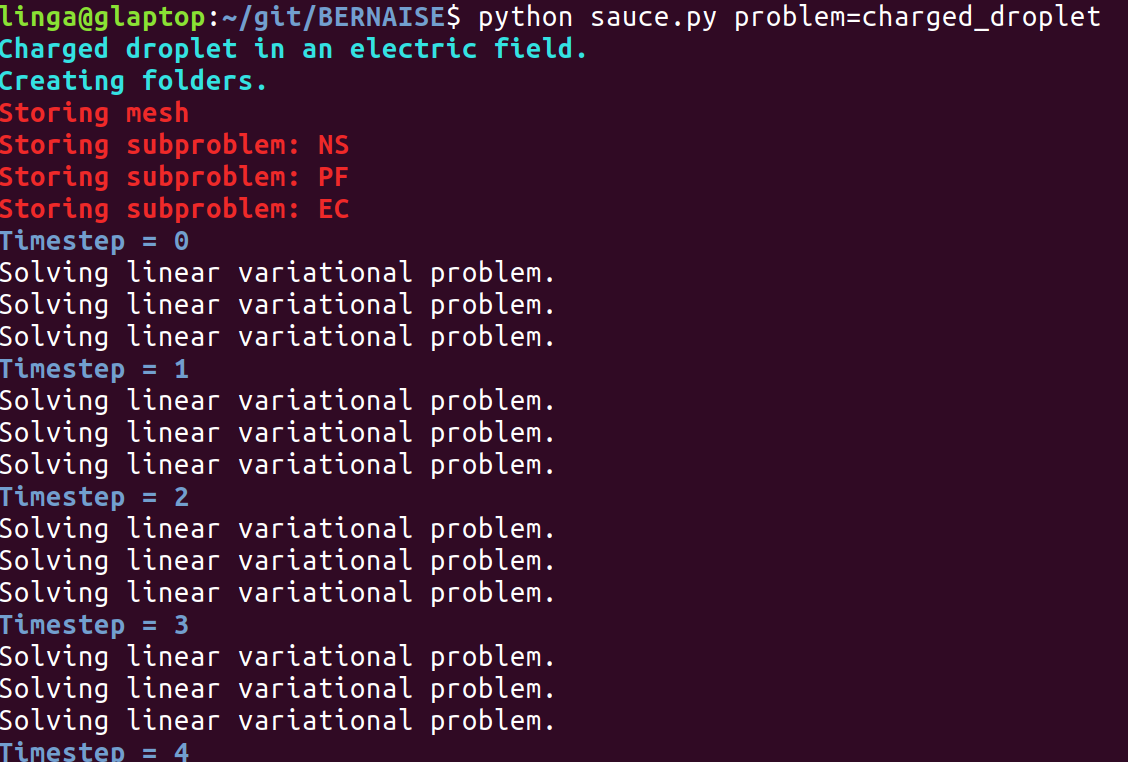
\includegraphics[width=0.75\textwidth]{charged_droplet_terminal.png}
  \caption{\label{fig:terminal}
    The charged droplet simulation seen from a Ubuntu terminal.
  }
\end{figure}
Now, to inspect the results we can, e.g., plot the physical fields after a certain time $t=8$.
We run:
\begin{minted}{bash}
>> python postprocess.py folder=results_charged_droplet/1/ \
   method=plot time=8 save=True
\end{minted}
The resulting plots for the phase field and for the velocity, that can be found in the folder \texttt{results\_charged\_droplet/1/Plots/}, are shown in Fig.\ \ref{fig:output}.
\begin{figure}
  \centering
  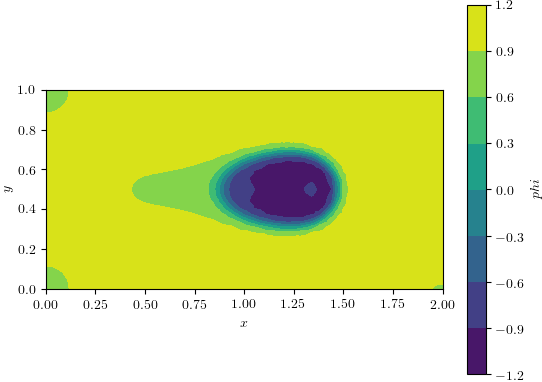
\includegraphics[width=0.75\textwidth]{phi_000020.png}\\
  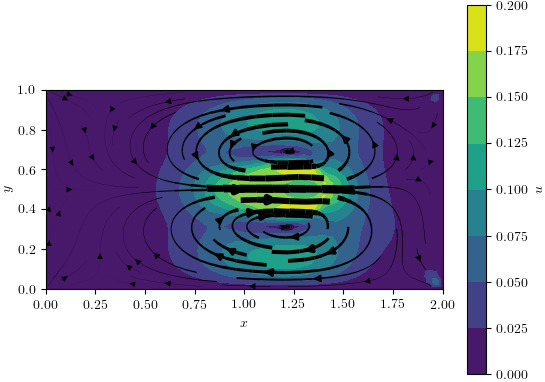
\includegraphics[width=0.75\textwidth]{u_000020.png}
  \caption{\label{fig:output}
    The charged droplet simulation.
    Top: phase field.
    Bottom: Velocity field.
    Note that this simulation is very coarse with large time steps (and thick interface), and therefore the phase field is somewhat smeared out.
  }
\end{figure}
The XDMF/HDF5 files can also be accessed and visualized directly using e.g.\ ParaView.

\bibliographystyle{abbrvnat}
\bibliography{references}

\end{document}